\documentclass{beamer}
\usepackage[english]{babel}
\usepackage[utf8]{inputenc}
\mode<presentation>{\usetheme{FS18}}
\usepackage{amsmath,amsthm, amssymb, latexsym}
\usepackage[orientation=portrait,size=a0,scale=1.4]{beamerposter}

\graphicspath{{../figures/graphics/}}
 
\title{A Continuous-Time Dynamical System Describing both Rate Encoding and Spiking Neurons}
\author{Fabian Schubert, Claudius Gros}
\institute{Institute for Theoretical Physics, Goethe University Frankfurt a.M.}
\date[Feb. 28th, 2018]{Feb. 28th, 2018}


\begin{document}
\begin{frame}[t]
\begin{columns}
\begin{column}{.45\textwidth}
\begin{block}{Introduction}
\begin{itemize}
\item We introduce a two-dimensional nonlinear system, modeling a wide range of dynamic 
properties of spiking neurons.
\item By altering key parameters of this system, its dynamics become identical to those of a 
time-continuous rate-encoding model.
\item Differences of the dynamical properties of single units as well as of network structures under 
these two regimes can be treated within the same mathematical framework.
\end{itemize}
\end{block}
\begin{block}{Neuron Model}
The model consists of a two-dimensional non-linear system given by
\begin{minipage}[t]{.5\linewidth}
\begin{align*}
\tau_x \dot{x} &= f(x) - y  \\ 
\tau_y \dot{y} &= g(x) - y 
\end{align*}
\end{minipage}%
\begin{minipage}[t]{.5\linewidth}
\begin{align*}
f(x) &= s \sigma \left(a\left(x-s/4\right)\right)  \\
g(x) &= g_0 \sigma\left(a_g\left(x-I\right)\right) - \Delta_y \\
\sigma(x) &= \left(1+\mathrm{exp}(-x)\right)^{-1}
\end{align*}
\end{minipage}
\begin{figure}
\centering
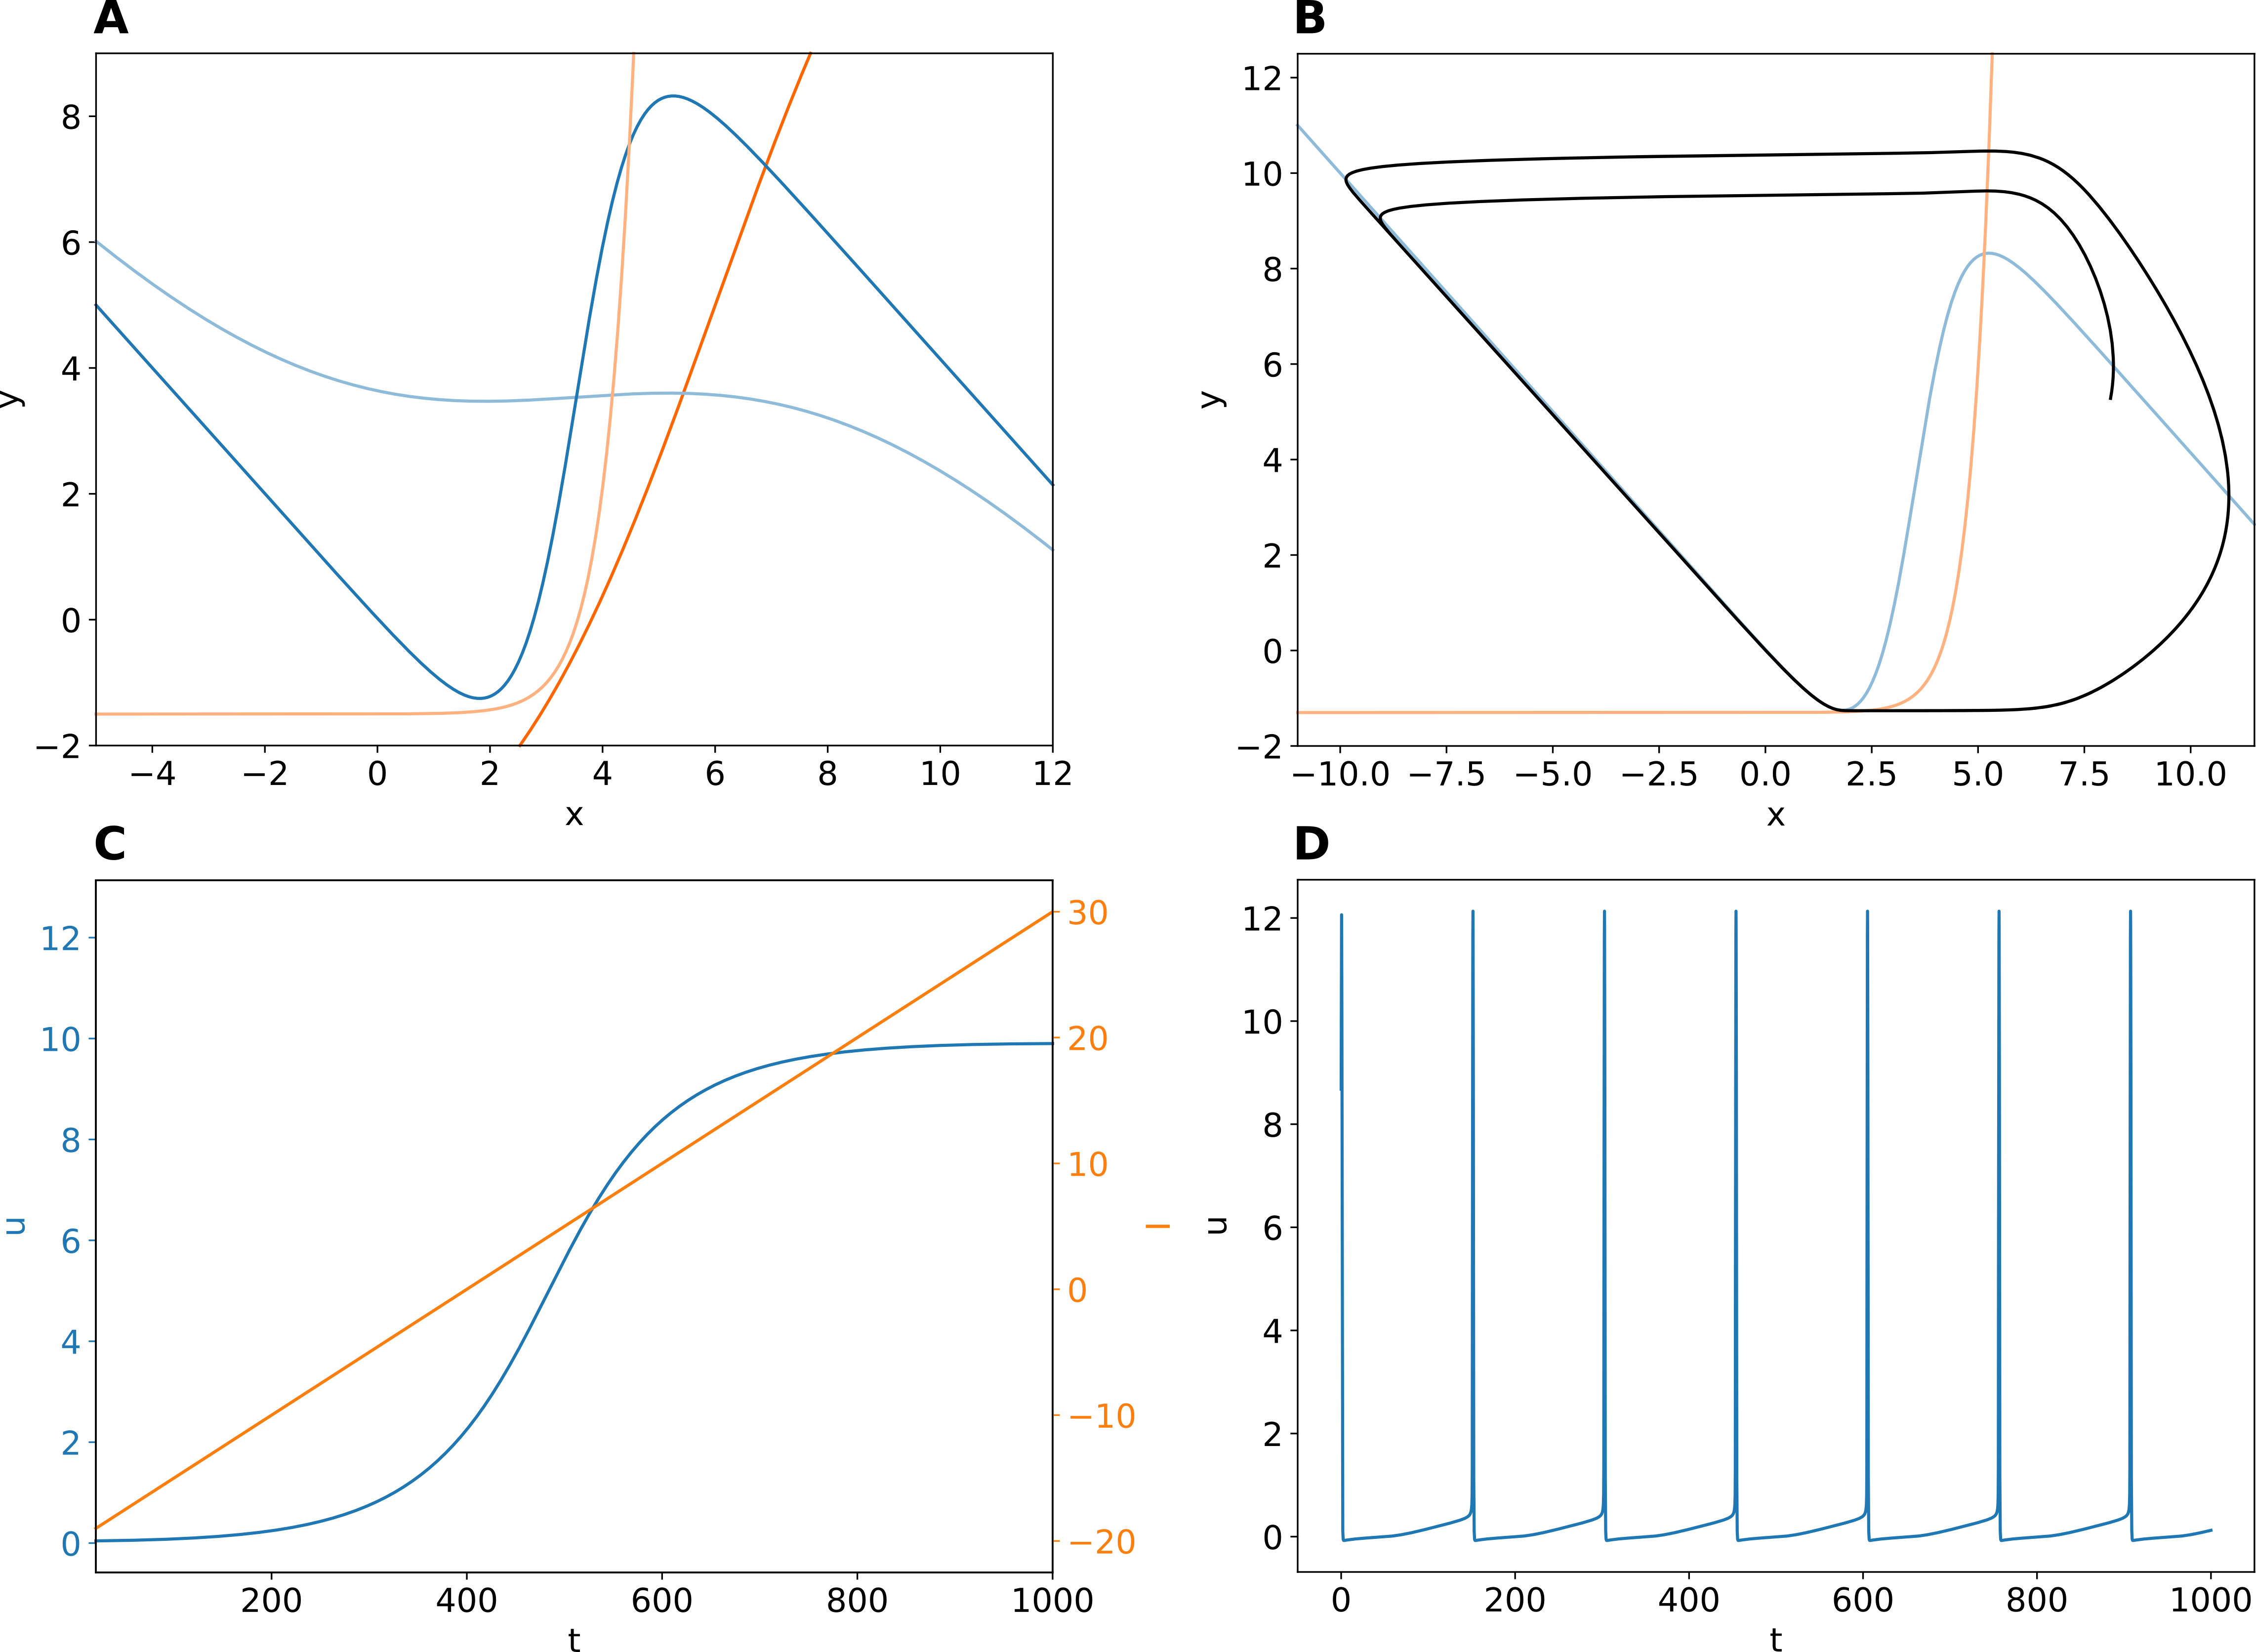
\includegraphics[width=0.8\textwidth]{../figures/graphics/dynamics_combined_figure.png}
\label{fig:dynamics_illustr}
\caption{A: x/y-nullclines (blue/red) of the dynamical system for parameter sets generating spiking/non spiking behavior. B: Phase plane trajectory for the spiking dynamics. C/D: Dynamics of readout variable $u$ for the spiking/non-spiking case.}
\end{figure}
\end{block}
\begin{block}{Results}
\begin{itemize}
\item A wide range of different types of spiking dynamics can be reproduced by this generic system.
\end{itemize}
\end{block}
\end{column}
\begin{column}{.45\textwidth}

\end{column}
\end{columns}
\end{frame}
\end{document}
